\chapter{Automatic differentiation}

\section{Introduction: differentiation methods}

Suppose that we have a function $f: \mathbb{R}^n \to \mathbb{R}^m$ that we want to differentiate.
We have many methods to do so:

\begin{enumerate}
    \item \textbf{Manual differentiation}: we can differentiate the function by hand.

    \begin{itemize}
        \item Pros: it is exact, fast, and good for theory
        \item Cons: it is error-prone, time-consuming, and difficult for complex functions
    \end{itemize}

    \item \textbf{Numerical differentiation}: we can approximate the derivative by finite differences.
    
    \begin{itemize}
        \item Pros: it is easy to implement
        \item Cons: it is slow, inaccurate (round-off and truncation errors), and not suitable for complex functions
    \end{itemize}

    Let us look at the example of finite differences in 1 dimension. We can formulate 3 ways to 
    approximate the derivative of a function $f: \mathbb{R} \to \mathbb{R}$ at a point $x$:

    \begin{itemize}
        \item Forward difference: $f'(x) \approx \frac{f(x + h) - f(x)}{h}$
        \item Backward difference: $f'(x) \approx \frac{f(x) - f(x - h)}{h}$
        \item Central difference: $f'(x) \approx \frac{f(x + h) - f(x - h)}{2h}$
    \end{itemize}

    The problem with the Finite Differences method (FDM) is that it presents two types of
    errors:

    \begin{itemize}
        \item \textbf{Truncation error}: it is the error that arises due to the approximation of the derivative.
        It is a consequence of the fact that we are using a Taylor series to approximate the derivative.
        This error decreases as $h$ decreases. For forward and backward differences, the error is $O(h)$, while
        for central differences, the error is $O(h^2)$.

        \item \textbf{Round-off error}: it is the error that arises due to the finite precision of the computer.
        It is a consequence of adding two numbers of different magnitudes, or subtracting two numbers that are 
        close to each other. This error increases as $h$ decreases. 
    \end{itemize}

    The following graph represents the trade-off between the truncation and round-off errors:

    \begin{figure}[H]
        \centering
        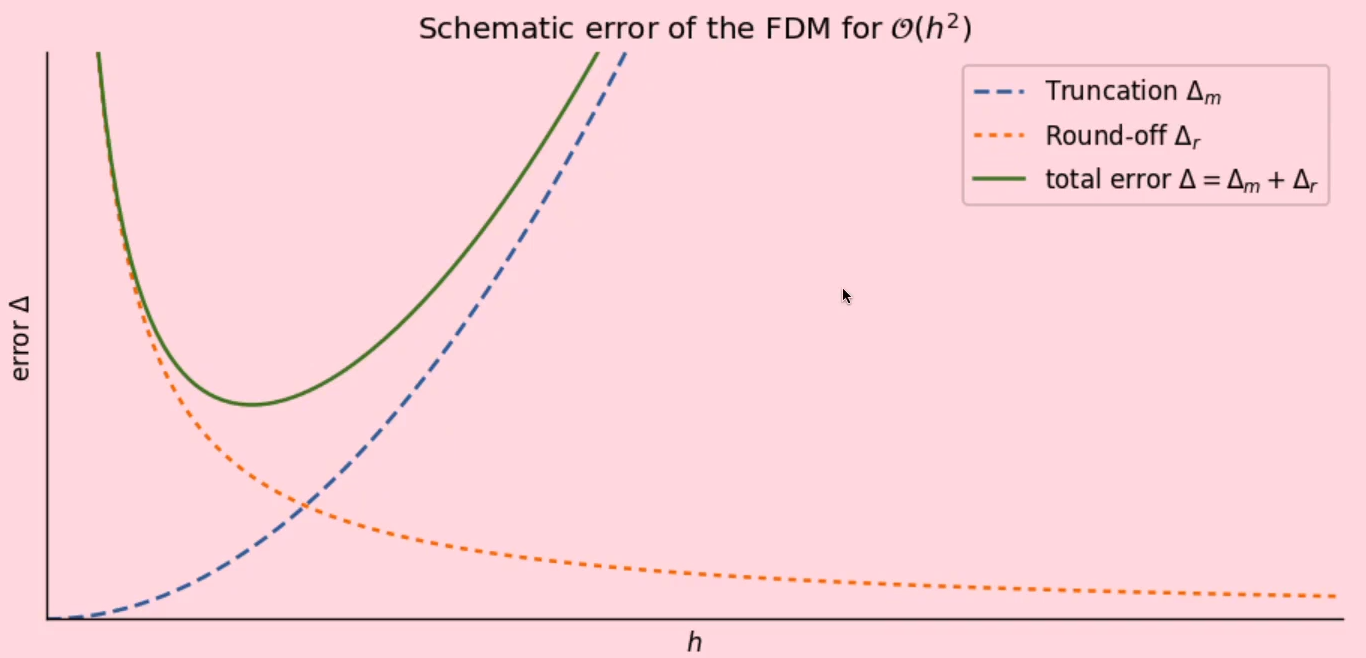
\includegraphics[width=0.6\textwidth]{figures/round-off_vs_trunc.png}
        \caption{Trade-off between truncation and round-off errors}
    \end{figure}

    And we can actually see this in an example:

    \begin{lstlisting}[language=Python]
import numpy as np

def forward_diff(f, x, h):
    return (f(x + h) - f(x)) / h

def centered_diff(f, x, h):
    return (f(x + h) - f(x - h)) / (2 * h)

h = np.logspace(-16, 0, num=500, endpoint=True)
x = 1.0
D1f = forward_diff(np.sin, x, h)
D2f = centered_diff(np.sin, x, h)
err1 = np.abs(D1f - np.cos(x))
err2 = np.abs(D2f - np.cos(x))
\end{lstlisting}

Then, the plot of the errors is:

\begin{figure}[H]
    \centering
    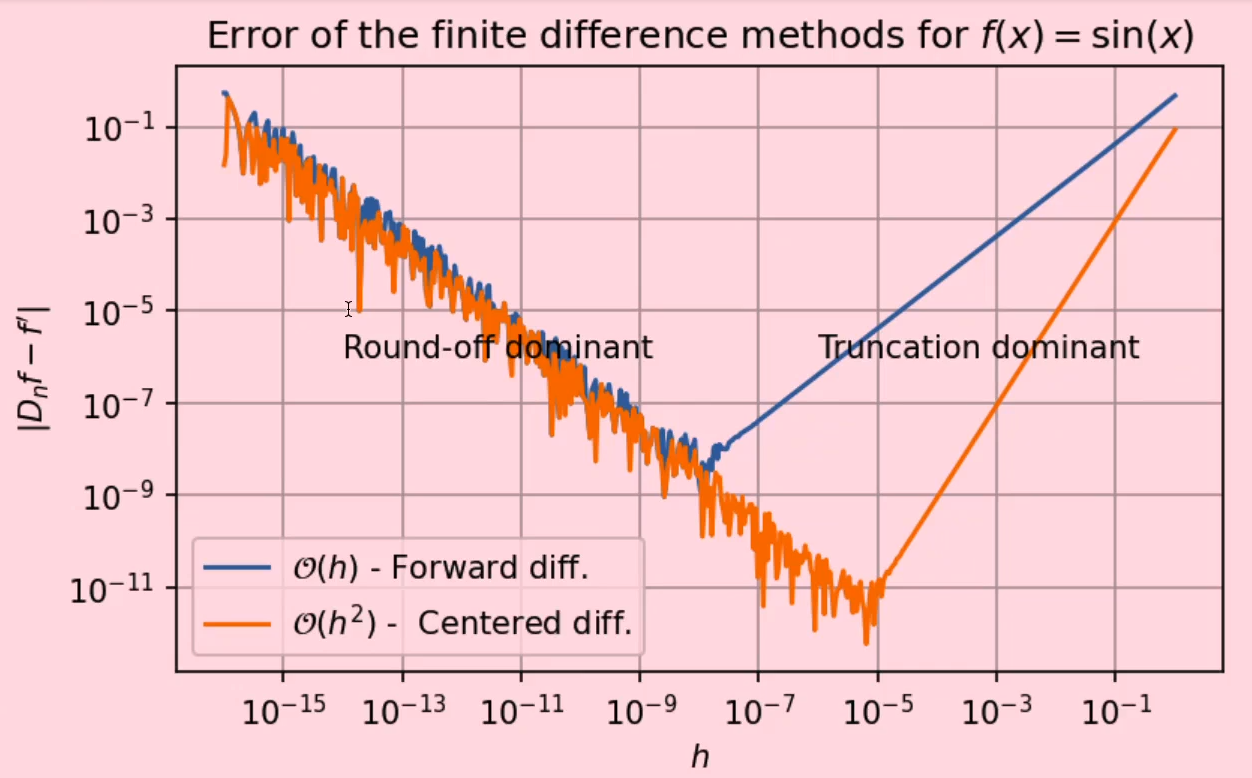
\includegraphics[width=0.6\textwidth]{figures/example_roundoff-trunc.png}
    \caption{Errors of the finite differences method}
\end{figure}

    \item \textbf{Symbolic differentiation}: we can use a computer algebra system (CAS) to compute the derivative symbolically.
    
    \begin{itemize}
        \item Pros: it is exact, good for theory.
        \item Cons: it is slow, memory-intensive, and can cause expression swell for complex functions.
    \end{itemize}

    \item \textbf{Automatic differentiation}: it is a technique that computes the derivative of a function by applying the chain rule.
    
    \begin{itemize}
        \item Pros: it is exact, fast, and general (good for complex functions).
        \item Cons: it is difficult to implement, and it requires a good understanding of the chain rule.
    \end{itemize}

\end{enumerate}

In this chapter, we will focus on automatic differentiation (AD). One of the main methods
of AD is the backward propagation algorithm, which is used in deep learning to compute the gradients
of the loss function with respect to the parameters of the model.\\

Automatic differentiation (AD) is a technique that it is based on the idea
of splitting the computation of the derivative of a function into elementary operations:

\begin{itemize}
    \item Unitary operations
    \item Exponentials, logarithms, trigonometric functions, etc.
\end{itemize}


\section{Automatic differentiation: Wengert list}

Automatic differentiation (AD) is a technique that computes the derivative of a function by applying the 
chain rule. It is based on the idea of splitting the computation of the derivative of a function into 
elementary operations. The main idea is to represent the function as a composition of elementary functions
and then apply the chain rule to compute the derivative.\\

To implement AD, we take advantage of the evaluation trace of the function, also called the forward primal
trace. This trace is a sequence of elementary operations that are applied to the input variables to compute
the output of the function. It keeps track of the intermediate values of the variables and the operations 
that are applied to them. These variables are called primal variables, and are typically denoted by $v_i$
for functions $f: \R^n \to \R^m$, following these rules:

\begin{itemize}
    \item \textbf{Input variables}: $v_{i-n} = x_i, \quad i = 1, ..., n$
    \item \textbf{Intermediate variables}: $v_i = g_i(v_{j_1}, ..., v_{j_k}), \quad i=1, ..., \ell, \quad j_i,...,j_k \subseteq [1-n, \ell]$
    \item \textbf{Output variables}: $y_{m-i} = v_{\ell - i}, \quad i = m-1, ..., 0$
\end{itemize}

For example, consider the function $f: \R^2 \to \R$ defined as $f(x, y) = \sin((x_1 + x_2) x_2^2)$. 
The evaluation trace of this function is:

\begin{itemize}
    \item $v_{-1} = x_1$, $v_{0} = x_2$
    \item $v_{1} = v_{-1} + v_{0}$
    \item $v_{2} = v_{0}^2$
    \item $v_{3} = v_{1} \cdot v_{2}$
    \item $v_{4} = \sin(v_{3})$
    \item $y_1 = v_4$
\end{itemize}

This trace is also called the Wengert list (as it was introduced by R. E. Wengert in 1964). We can represent
the Wengert list as a directed acyclic graph (DAG), where nodes represent variables and edges
describe the computational hierarchy of input to output transformations. This graph is also commonly
referred to as the computational graph. For the previous example, we get:

\begin{figure}[H]
    \centering
    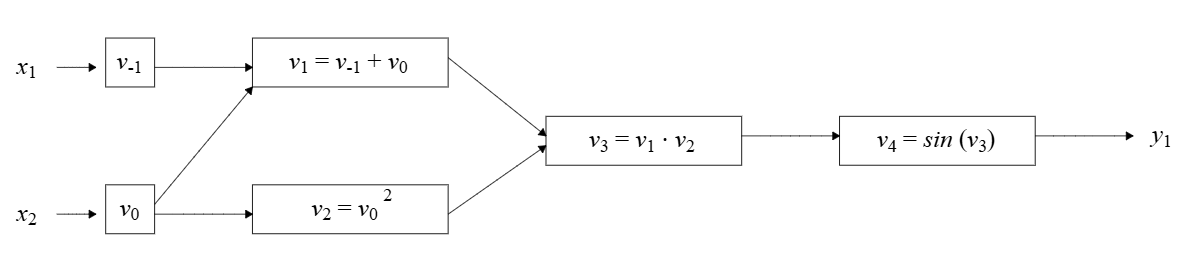
\includegraphics[width=0.95\textwidth]{figures/DAG_autodiff.png}
    \caption{Comp. graph of the function $f(x, y) = \sin((x_1 + x_2) x_2^2)$}
    \label{fig:DAG_autodiff}
\end{figure}

These tools are essential for the implementation of AD, in particular, its two modes:

\begin{itemize}
    \item \textbf{Forward mode}
    \item \textbf{Backward mode}
\end{itemize}

\section{Forward mode of AD}

The forward mode of automatic differentiation (AD) adopts the idea of the evaluation trace,
but introduces a new concept: the tangent variables, usually denoted by $\dot{v}_i$. These
tangents carry the derivative information of the primal variables with respect to a single
input variable of interest. For example, if we are interested in computing the derivative
of a function $f: \R^n \to \R^m$ with respect to the variable $x_i$, we write:

$$\dot{v}_j = \frac{\partial v_j}{\partial x_i} \quad j = 1-n, ..., \ell$$

The forward mode of AD computes the derivative of a function by applying the chain rule
to the evaluation trace. It is based on the idea of propagating the derivative information
from the input variables to the output variables. For this, we calculate what is called
the forward tangent trace, by simply applying derivation rules to the evaluation trace.
For example, consider the same function $f(x, y) = \sin((x_1 + x_2) x_2^2)$.
The forward tangent trace of this function is:

\begin{itemize}
    \item $\dot{v}_{-1} = \dot{x}_1$, $\dot{v}_{0} = \dot{x}_2$
    \item $\dot{v}_{1} = \dot{v}_{-1} + \dot{v}_{0}$
    \item $\dot{v}_{2} = 2 v_{0} \dot{v}_{0}$
    \item $\dot{v}_{3} = v_{2} \dot{v}_{1} + v_{1} \dot{v}_{2}$
    \item $\dot{v}_{4} = \cos(v_{3}) \dot{v}_{3}$
    \item $\dot{y}_1 = \dot{v}_4$
\end{itemize}

In general, by following the computational graph, we can propose the following formula for
the tangent variables:

\begin{equation}
    \dot{v}_i = \sum_{j \in \{\text{predecesors of } i\}} \frac{\partial v_i}{\partial v_j} \dot{v}_j
\end{equation}

In the case of the input variables (that don't have predecesors), we notice that the tangent
variables, by definition, are always either 0 or 1. This is because the input variables 
are independent of each other, so their derivatives are 0, except for the variable 
of interest, which has a derivative of 1, as it is the variable with respect to which 
we are computing the derivative.\\

In fact, by setting the tangent variables of the input variables to 0 or 1, we can compute
the derivative of the function with respect to any input variable, following the forward 
tangent trace. This is the main idea of the forward mode of AD.\\

For example, let us calculate the derivative of the previous function in the point
$(x, y) = (1, 2)$ with respect to the variable $x_1$. We can do this by setting the
tangent variables of the input variables to 0 or 1, as well as the primal input variables
to their values at the point $(1, 2)$. Then, we can compute the forward primal and
tangent traces to get the derivative of the function with respect to $x_1$:

\begin{table}[H]
    \centering
    \begin{tabular}{@{}l|lc|l|l@{}}
        \toprule
        \textbf{Forward Primal Trace} & \textbf{Output}   & \phantom{a} & \textbf{Forward Tangent Trace}                & \textbf{Output}             \\ \midrule
        $v_{-1} = x_1$               & 1                  &             & $\dot{v}_{-1} = \dot{x}_1$                    & 1                           \\
        $v_0 = x_2$                  & 2                  &             & $\dot{v}_0 = \dot{x}_2$                       & 0                           \\ \midrule
        $v_1 = v_{-1} + v_0$         & $1 + 2 = 3$        &             & $\dot{v}_1 = \dot{v}_{-1} + \dot{v}_0$        & $1 + 0 = 1$                 \\
        $v_2 = v_0^2$                & $2^2 = 4$          &             & $\dot{v}_2 = 2 v_0 \cdot \dot{v}_0$           & $2 \cdot 2 \cdot 0 = 0$     \\
        $v_3 = v_1 \cdot v_2$        & $3 \cdot 4 = 12$   &             & $\dot{v}_3 = v_2 \dot{v}_1 + \dot{v}_2 \cdot v_1$ & $4 \cdot 1 + 0 \cdot 3 = 4$ \\ 
        $v_4 = \sin v_3$             & $\sin(12) = -0.54$ &             & $\dot{v}_4 = \cos(v_3) \cdot \dot{v}_3$       & $\cos(12) \cdot 4 = 3.38$   \\ \midrule
        $y_1 = v_4$                  & $-0.54$            &             & $\dot{y}_1 = \dot{v}_4$                       & 3.38                        \\ \bottomrule
    \end{tabular}
    \caption{Example of forward mode of AD}
\end{table}

The same can be done, setting the tangent variable $\dot{v}_0 = 1$, to compute the derivative
of the function with respect to $x_2$. The result is $\dot{y}_1 = -13.501$. So in the end,
we have computed the derivative of the function with respect to $x_1$ and $x_2$ at the point
$(1, 2)$, which is $3.38$ and $-13.501$, respectively.\\

This process is the essence of forward mode AD. At every elementary operation for a given 
function, compute intermediate variables (primals) by applying basic arithmetic operations, 
and in synchrony, compute their derivatives (tangents).\\

We can generalize this procedure to compute Jacobians of functions $f: \R^n \to \R^m$ evaluated
at a point $x_0 \in \R^n$. Remember that the Jacobian is a matrix that contains the partial
derivatives of the function with respect to each input variable:

\begin{equation}
    J_f(x_0) = \begin{bmatrix}
        \frac{\partial f_1}{\partial x_1} & \cdots & \frac{\partial f_1}{\partial x_n} \\
        \vdots & \ddots & \vdots \\
        \frac{\partial f_m}{\partial x_1} & \cdots & \frac{\partial f_m}{\partial x_n}
    \end{bmatrix}
\end{equation}
\vspace{1em}

To compute the Jacobian of a function $f: \R^n \to \R^m$ evaluated at a point $x_0 \in \R^n$,
we can use the forward mode of AD. We set the input variables to $x_0$, and the tangent variables
equal to the canonical basis vectors $e_i$ of $\R^n$, for $i = 1, ..., n$. Every pass through
the forward mode of AD for each $e_i$ will give us the $i$-th column of the Jacobian.\\

Because the function $f: \R^n \to \R^m$ has $n$ input variables, we need to perform $n$ passes
through the forward mode of AD to compute the Jacobian. So this procedure has a complexity of
$O(n)$. This is the main drawback of the forward mode of AD: it is not efficient for functions
with a large number of input variables, with respect to the output variables, i.e., $n \gg m$.\\

\subsection{Note: Forward mode and Jacobian-vector product (JVP)}

In practice, we are often interested in computing the product of the Jacobian of a function
$f: \R^n \to \R^m$ evaluated at a point $x_0 \in \R^n$ with a vector $r \in \R^n$. This operation
is called the Jacobian-vector product, and it is denoted by $J_f(x_0) \cdot r$.\\

The Jacobian-vector product can be computed using the forward mode of AD. We set the input variables
to $x_0$, and the tangent variables equal to $r$. Then, a single pass through the forward mode of AD
will give us the product of the Jacobian with the vector $r$. This is a more efficient way to compute
the Jacobian-vector product, and sometimes it is more convenient than computing the full Jacobian.

\section{Backward mode of AD}

Backward mode of automatic differentiation (AD), also known as reverse mode of AD, is a technique
that computes the derivative of a function by applying the chain rule in reverse order. It is based
on the idea of propagating the derivative information from the output variables to the input variables.\\

This method introduces a new concept: the adjoint variables, usually denoted by $\bar{v}_i$. These
adjoints carry the derivative information of a single output variable with respect to a variable
(intermediate or input) of interest. For example, if we are interested in computing the derivative
of the output variable $y_j$ with respect to the variable $v_i$, we write:

$$\bar{v}_i = \frac{\partial y_j}{\partial v_i} \quad i = 1-n, ... \ell$$

As in forward mode, in reverse mode we also perform a pass through the evaluation trace of the function.
But this time, the adjoint variables are not computed alongside the primal variables. Instead, we store
any dependency information that is needed to compute the adjoints in the computational graph (Wengert list).
Then we perform a backward pass through the computational graph to compute the adjoints.\\

Given the computational graph, the adjoint variables can be computed by the following formula:

\begin{equation}
    \bar{v}_i = \sum_{j \in \{\text{successors of } i\}} \frac{\partial v_j}{\partial v_i} \bar{v}_j
\end{equation}

In the case of the output variables (that don't have successors), we notice that the adjoint variables
are always either 0 or 1. This is because, by definition, the adjoint of the output variables are calculated
with respect to the output variables, so their derivatives are 0, except for the variable of interest, which
has a derivative of 1, as it is the variable with respect to which we are computing the derivative.\\

Notice that when we reach to the input variables, we have computed the derivative of the function with respect
to all the output variables. This is the main idea of the backward mode of AD. At every elementary operation
for a given function, compute intermediate variables (primals) by applying basic arithmetic operations, and
store any dependency information that is needed to compute the adjoints. Then, perform a backward pass through
the computational graph to compute the adjoints.\\

For example, consider the same function $f(x, y) = \sin((x_1 + x_2) x_2^2)$. The computational graph of this
function is shown in Figure \ref{fig:DAG_autodiff}. The adjoint trace of this function is:

\begin{itemize}
    \item $\bar{y}_1 = 1$
    \item $\bar{v}_4 = 1 \cdot \bar{y}_1$
    \item $\bar{v}_3 = \cos(v_3) \cdot \bar{v}_4$
    \item $\bar{v}_2 = \bar{v}_3 \cdot v_1$
    \item $\bar{v}_1 = \bar{v}_3 \cdot v_2$
    \item $\bar{v}_0 = 2 v_0 \cdot \bar{v}_2 + 1 \cdot \bar{v}_1$
    \item $\bar{v}_{-1} = 1 \cdot \bar{v}_1$
\end{itemize}

For the same example, let us calculate the derivative of the function in the point $(x, y) = (1, 2)$:

\begin{table}[H]
    \centering
    \begin{tabular}{@{}l|lc|l|l@{}}
        \toprule
        \textbf{Forward Primal Trace} & \textbf{Output}   & \phantom{a} & \textbf{Backward Adjoint Trace}                & \textbf{Output}             \\ \midrule
        $v_{-1} = x_1$               & 1                  &             & $\bar{v}_{-1} = 1 \cdot \bar{v}_1$             & $3.375$                           \\
        $v_0 = x_2$                  & 2                  &             & $\bar{v}_0 = 2 v_0 \cdot \bar{v}_2 + 1 \cdot \bar{v}_1$ & $4 \cdot 2.351 + 3.375 = 13.501$ \\ \midrule
        $v_1 = v_{-1} + v_0$         & $1 + 2 = 3$        &             & $\bar{v}_1 = \bar{v}_3 \cdot v_2$              & $0.843 \cdot 4 = 3.375$      \\
        $v_2 = v_0^2$                & $2^2 = 4$          &             & $\bar{v}_2 = \bar{v}_3 \cdot v_1$              & $0.843 \cdot 3 = 2.531$      \\
        $v_3 = v_1 \cdot v_2$        & $3 \cdot 4 = 12$   &             & $\bar{v}_3 = \cos(v_3) \cdot \bar{v}_4$        & $\cos(12) \cdot 1 = 0.843$   \\
        $v_4 = \sin v_3$             & $\sin(12) = -0.54$ &             & $\bar{v}_4 = 1 \cdot \bar{y}_1$                & 1                           \\ \midrule
        $y_1 = v_4$                  & $-0.54$            &             & $\bar{y}_1 = 1$                                & 1                           \\ \bottomrule
    \end{tabular}
    \caption{Example of backward mode of AD}
\end{table}

Notice that the result of the derivative of the function with respect to $x_1$ and $x_2$ at the point
$(1, 2)$ is the same as in the forward mode of AD. But in this case, we only needed to perform a single
pass through the computational graph to compute the derivatives.\\

As well as in the forward mode of AD, we can generalize this procedure to compute Jacobians of functions
$f: \R^n \to \R^m$ evaluated at a point $x_0 \in \R^n$. We just need to set the input variables to $x_0$ for
the evaluation trace, and the adjoint output variables to the canonical basis vectors $e_i$ of $\R^m$, 
for $j = 1, ..., m$. Then, perform a single pass through the computational graph to compute the Jacobian. 
For each $e_i$, we will get the $i$-th row of the Jacobian.\\

Because the function $f: \R^n \to \R^m$ has $m$ output variables, we need to perform $m$ passes through the
backward mode of AD to compute the Jacobian. So this procedure has a complexity of $O(m)$. This is the main
advantage of the backward mode of AD: it is more efficient for functions with a large number of output variables,
with respect to the input variables, i.e., $n \gg m$, which is usually the case in deep learning.

\subsection{Note: Backward mode and vector-Jacobian product (VJP)}

In practice, we are often interested in computing the product of a vector $r \in \R^m$ with the Jacobian of a
function $f: \R^n \to \R^m$ evaluated at a point $x_0 \in \R^n$. This operation is called the vector-Jacobian
product, and it is denoted by $r^T \cdot J_f(x_0) = J_f(x_0)^T \cdot r$.\\

In the same way as in the forward mode of AD, the vector-Jacobian product can be computed using the backward mode
of AD. We set the input variables to $x_0$ for the evaluation trace, and the adjoint output variables to $r$.
Then, a single pass through the computational graph will give us the product of the vector $r^T$ with the Jacobian.
This is a more efficient way to compute the vector-Jacobian product, and sometimes it is more convenient than
computing the full Jacobian.


\section{Dual numbers}

We define a dual number as a pair of real numbers $(a, b)$, where $a$ is the real part, and $b$ is the dual part.
It is expressed as follows:

\begin{equation}
    z = a + b \varepsilon
\end{equation}

where $\varepsilon$ is a number such that $\varepsilon \neq 0 \; \wedge \; \varepsilon^2 = 0$. 
We can define the operations of addition and multiplication as follows:

\begin{itemize}
    \item Addition: 
    $$(a + b \varepsilon) + (c + d \varepsilon) = (a + c) + (b + d) \varepsilon$$

    \item Multiplication: 
   $$(a + b \varepsilon) \cdot (c + d \varepsilon) = ac + (ad + bc) \varepsilon$$

\end{itemize}

Now, let us consider a generic function $f(\cdot)$. We will evaluate the function in a 
dual number $z = x + \varepsilon$. We can expand the function in a Taylor series around $x$:

\begin{equation}
    f(z) = f(x + \varepsilon) = f(x) + f'(x) \varepsilon + O(\varepsilon^2)
\end{equation}

Because $\varepsilon^2 = 0$, we have that:

\begin{equation}
    f(z) = f(x) + f'(x) \varepsilon
\end{equation}

This means that the dual part of the function evaluated in a dual number is the derivative of the function
evaluated at the real part of the dual number. This is the key idea behind the dual numbers: we can use them
to compute the derivative of a function by evaluating the function in a dual number.\\

Let us expand the idea to a general dual number $a + b \varepsilon$. We can evaluate the function $f(\cdot)$
in the dual number as follows:

\begin{equation}
    f(a + b \varepsilon) = f(a) + f'(a) b \varepsilon
\end{equation}

With this property, we can also compute the derivative of a composite function. Suppose that we 
have two functions $f(\cdot)$ and $g(\cdot)$. We can compute the derivative of the composite 
function $h(\cdot) = f(g(\cdot))$ as follows:

\begin{equation}
    h(x + \varepsilon) = f(g(x + \varepsilon)) = f(g(x) + g'(x) \varepsilon) = f(g(x)) + f'(g(x)) g'(x) \varepsilon
\end{equation}

This means that we can compute the derivative of a composite function by evaluating the functions 
in dual numbers.\\

We can also redefine the dual numbers to obtain the second derivative of a function. We just need to
define $\varepsilon^2 \neq 0$ and $\varepsilon^3 = 0$. 
